\chapter{The Flawed Human Brain}
\bichaptertitle{有缺陷的人类大脑}

\noindent\textsc{Human minds can do wonderful things, but are deeply flawed when making
financial decisions.} In this chapter I explore economic theories about human behaviour,
and why systematic trading and investing makes sense. I also show how our irrationality
can interfere with the design of systematic strategies.

\noindent\textbf{人类心智能够完成许多了不起的事情，但在做金融决策时却存在根深蒂固的缺陷。} 在本章中，我会探讨经济学中关于人类行为的理论，
说明为什么系统化交易与投资是有道理的。我也会展示，我们的非理性会如何干扰系统化策略的设计。

\section*{Chapter overview}
\phantomsection
\addcontentsline{toc}{section}{Chapter overview}
\bisectiontitle{本章概览}

\begin{tabularx}{\textwidth}{@{}p{0.3\textwidth}Y@{}}
\textbf{Humans should be great traders, but...} & The research that tells us why humans make
bad decisions. \\
\textbf{Simple trading rules} & The dumb systems that are better at investing and trading
than clever humans. \\
\textbf{Sticking to the plan} & Why you must be committed to your systems for them to
work. \\
\textbf{Good system design} & Avoiding the human failings which can still be dangerous
when designing systematic trading strategies. \\
\end{tabularx}

\medskip

\begin{tabularx}{\textwidth}{@{}p{0.3\textwidth}Y@{}}
\textbf{人类本应是出色的交易者，但是……} & 解释人类为何会做出糟糕决策的研究。 \\
\textbf{简单交易规则} & 那些看起来很笨，却比聪明人更擅长投资和交易的系统。 \\
\textbf{坚持计划} & 为什么你必须真正承诺并遵守自己的系统，它们才会发挥作用。 \\
\textbf{良好的系统设计} & 在设计系统化交易策略时，如何避开那些依旧可能带来危险的人性弱点。 \\
\end{tabularx}

\section*{Humans should be great traders, but...}
\phantomsection
\addcontentsline{toc}{section}{Humans should be great traders, but...}
\bisectiontitle{人类本应是出色的交易者，但是……}

Why do we need to trade or invest in a systematic fashion? What is wrong with using our
own intuition to trade in a discretionary way? After all our brains have an astonishing
ability to absorb and react to complex data, like those we see in financial markets. In my
own Barclays trade described in the introduction I did analysis that would be virtually
impossible to replicate with a systematic rule. But a simple rule would have been more
successful than I was.\footnote{If in 2009 I had developed the idea of semi-automatic
trading then I could have taken more advantage of my uncharacteristically brilliant
analysis, by putting the trade on in a framework which controlled my risk properly.\par 如果我在 2009 年就已经形成了半自动交易的理念，
那么我本可以把那次少见的精彩分析更充分地利用起来，把交易放进一个能够正确控制风险的框架中执行。}

为什么我们需要以系统化的方式进行交易或投资？依赖自己的直觉、用主观判断去交易，到底有什么问题？毕竟，我们的大脑拥有惊人的能力，
可以吸收并回应复杂的数据，就像金融市场中那些纷繁的信息一样。在导言里我讲到自己做巴克莱交易时，所做的分析几乎不可能通过一条系统化规则完整复制出来。
但即便如此，一条简单规则的表现仍然会比我更好。

Unfortunately there have been many other times when a systematic strategy would have
made better decisions than I did. For example in 2004 I bought some shares in UK oil
company BP. They quickly rose about 5\% and I sold them for a small profit. They
subsequently rallied to a much higher level. I resolved never to sell too quickly again.
Then in late 2009 I decided to recycle some of my Barclays profits into buying BP.
Initially they went from \pounds 5 to over \pounds 6. But in April 2010 one of BP's
drilling rigs exploded in devastating fashion, killing 11 people. The shares started to fall,
and a month later they were back at \pounds 5. Scarred by my earlier experience I hung
on, convinced they would rebound. I finally sold at \pounds 3, which turned out to be the
bottom.

遗憾的是，还有许多其他时候，系统化策略本可以做出比我更好的决定。比如 2004 年，我买入了英国石油公司 BP 的一些股票。它们很快上涨了大约 5\%，
于是我小赚一笔便卖掉了。结果后来股价继续大涨，升到了更高的位置。我因此下定决心，以后绝不再那么快卖出。接着到了 2009 年底，我决定把一部分巴克莱交易赚到的钱，
重新投入到 BP 上。起初股价从 5 英镑涨到了 6 英镑以上。但到了 2010 年 4 月，BP 的一座钻井平台发生灾难性爆炸，造成 11 人死亡。股价开始下跌，
一个月后又跌回了 5 英镑。由于之前卖太早的经历让我留下了阴影，我选择继续死扛，坚信它一定会反弹。最后我在 3 英镑时卖出，而那恰恰是最低点。

I got it wrong both times. Was this just bad luck --- a BP jinx? Am I a particularly poor
trader, or is this evidence of a deeper problem with human psychology?

这两次我都做错了。这仅仅是运气不好 --- 好像中了 BP 的邪？是因为我特别不擅长交易，还是说这其实反映了人类心理更深层次的问题？

In fact despite their awesome complexity human brains like mine, and yours, are
fundamentally flawed. In the jargon they are subject to cognitive biases which result in
irrational behaviour. These instincts are so strong they mostly overwhelm any natural
advantage that humans should have over simple decision-making rules. To see why this
happens we need to understand how economists have tried to model and understand
human behaviour.

事实上，尽管人脑复杂得令人惊叹，不论是我的还是你的，都在根本上存在缺陷。用术语来说，我们会受到认知偏差的影响，从而表现出非理性行为。
这些本能如此强大，以至于它们往往会压倒人类相对于简单决策规则本应拥有的任何天然优势。要理解为什么会这样，我们就需要先弄清楚经济学家是如何尝试建模和理解人类行为的。

\subsection*{The death of rational economic man}
\bisubsectiontitle{理性经济人的终结}

When the ideas of classical finance were developed in the 1950s economists assumed
that people behaved in a purely rational way, resulting in perfectly efficient markets.
Over time many apparent anomalies in this theory were discovered. But these were
easily dismissed by the academic establishment as irrelevant, statistically insignificant
or explainable through some combination of risk factors. Crucially nobody was able to
come up with an alternative model that was as self-consistent and elegant as the efficient
markets hypothesis.

20 世纪 50 年代，经典金融学理论形成之时，经济学家假设人们会以纯粹理性的方式行事，因此市场将是完全有效的。随着时间推移，
这一理论中许多看似异常的现象被陆续发现。但学术主流很容易就把这些现象斥为无关紧要、统计上不显著，或者只是某种风险因子组合的结果。更关键的是，
始终没有人能提出一个像有效市场假说那样既自洽又优雅的替代理论模型。

From the 1980s onwards the field was penetrated by researchers from the discipline of
psychology. For these experts in the human mind, the economist's framework of pure
rationalism must have been highly amusing. A key insight these academic interlopers
brought was that our brains are loaded with baggage from the distant past.

从 20 世纪 80 年代开始，这一领域受到了心理学研究者的“入侵”。对于这些研究人类心智的专家来说，经济学家那套纯理性框架想必显得颇为可笑。
这些“跨界闯入者”带来的一个关键洞见是：我们的头脑背负着许多来自遥远过去的包袱。

Parts of our grey matter are still hardwired for survival in a hostile environment where
quick thinking was better than slow thoughtful consideration. As a result we have
deep-rooted instincts that make it extremely difficult to behave in the rational way that
classical finance expects. The new field that the interlopers created was behavioural
finance, and it did have its own unifying model: prospect theory.

我们大脑中的某些部分，至今仍然是为了在恶劣环境中求生而“硬编码”出来的；在那样的环境里，快速反应往往比缓慢而周密的思考更有优势。
结果就是，我们拥有许多根深蒂固的本能，使得我们极难按照经典金融学所期待的那种理性方式行事。这些“入侵者”开创出来的新领域就是行为金融学，
而它确实有自己的统一模型：前景理论。

\subsection*{Why we run losses and stop out profits}
\bisubsectiontitle{为什么我们会死扛亏损、过早止盈}

Prospect theory explains why investors get it wrong when confronted with certain trading
decisions, such as whether to sell out of a position which is now showing a loss. Most
people show the greatest reluctance to take losses, as I did in 2010 with BP.\footnote{For
more academic detail see for example Terence Odean, ``Are Investors Reluctant To Realize
Their Losses?'', \textit{Journal of Finance} 1998.\par 更详细的学术讨论可参见 Terence Odean 于 1998 年发表于 \textit{Journal of Finance}
的论文 “Are Investors Reluctant To Realize Their Losses?”。}

前景理论解释了为什么投资者在面对某些交易决策时会犯错，比如是否该卖掉一个已经浮亏的头寸。大多数人在止损这件事上都会表现出极大的抗拒，
我在 2010 年处理 BP 时就是如此。

This has been catchily described as ``get-evenitis'' by Hersh Shefrin.\footnote{Shefrin
2007, \textit{Beyond Greed and Fear}. I highly recommend this book for a clear overview
of behavioural finance, despite its age. In academic circles this is the ``disposition effect''
described in Shefrin and Statmen, ``The disposition to sell winners too early and ride
losers too long: theory and evidence'', \textit{Journal of Finance} 1985.\par Shefrin 在 2007 年出版的 \textit{Beyond Greed and Fear}
中把这种现象形象地称作 “get-evenitis（回本执念）”。尽管这本书年代较早，但我仍非常推荐它，因为它对行为金融学做了清晰的概述。
在学术界，这对应的是 Shefrin 和 Statmen 在 1985 年发表于 \textit{Journal of Finance} 的论文中所描述的 “disposition effect（处置效应）”。}
This aversion to taking losses is a very powerful instinct. Humans do not seem to view a
paper loss as real until it has been crystallised, so we can postpone the painful feeling of losing money. We
are also reluctant to admit that we made a mistake with our initial purchase. Selling is an
admission of failure.

Hersh Shefrin 把这种现象形象地称为 “get-evenitis”，也就是一种执着于回本的病症。对止损的厌恶是一种极其强烈的本能。
人类似乎并不会把浮亏真正当成现实损失，直到它被最终实现，因此我们可以把亏钱的痛苦感受往后拖延。我们也不愿承认自己最初买入时犯了错。
卖出，就意味着承认失败。

Conversely, if a position has risen in value we are happy to take profits and sell quickly,
as in my 2004 BP trade. The main motivation behind selling positions at a small profit
appears to be to minimise regret. If the stock fell back after reaching a new high we would
castigate ourselves for not taking profits earlier. Selling also confirms that our initial buy
decision was correct. We hunger to get that confirmation as quickly as possible.

反过来，如果一个头寸已经上涨了，我们就会乐于迅速止盈离场，就像我在 2004 年做 BP 时那样。以小利润卖出头寸背后的主要动机，
似乎是为了最小化后悔。如果股票在创新高之后又跌回去，我们就会责怪自己为何没有更早兑现利润。卖出还会确认我们最初买入的决定是正确的。
我们渴望尽快得到这种确认。

Both of these effects are at odds with classical financial theory, which says that people's
actions and preferences for risk are unrelated to whether they have made paper profits or
losses. In contrast prospect theory says we take more risks in a losing position to get even,
but we want less risk when winning, preferring a quick and certain gain to a chance of
losing our profits.

这两种效应都与经典金融理论相矛盾。经典理论认为，人们的行为以及对风险的偏好，不应当和自己当前是浮盈还是浮亏有关。相反，前景理论认为，
当处于亏损状态时，人们会为了回本而承担更多风险；而当处于盈利状态时，人们则更希望降低风险，宁愿要一个快速而确定的收益，也不愿冒把已有利润再亏回去的风险。

Unfortunately taking small profits and letting losses run is almost always a bad idea. I can
show you this by back-testing a trading system which mimics someone taking profits on
small rises, but allowing losses to grow larger before cutting --- an ``early profit
taker''.\footnote{This is based on the ``A and B'' system defined in appendix B with
parameters A = 5 and B = 20.\par 这基于附录 B 中定义的 “A and B” 系统，其中参数 A = 5，B = 20。}
A back-test shows how profitable this rule would have
been if it had been run in the past. Figure 2 shows part of the back-test and illustrates
how the rule would have traded treasury futures during summer 2011, when the USA's
sovereign debt rating was downgraded causing a counter intuitive rally. It sells and goes
short in early June on a small profit and then misses the subsequent rise in prices.

遗憾的是，过早止盈而任由亏损扩大，几乎总是个坏主意。我可以通过回测一套交易系统来说明这一点。这个系统模仿的是一种人在价格稍有上涨时就获利了结，
但会先容忍亏损继续扩大、等到更大亏损时才止损的行为，我把它叫作“过早止盈者（early profit taker）”。回测可以展示，如果过去运行这条规则，它会有多赚钱。
图 2 展示了这项回测的一部分，说明在 2011 年夏天美国主权债评级被下调、反而引发美债价格反直觉上涨时，这条规则会如何交易国债期货。它在 6 月初小赚后卖出并反手做空，
结果错过了后续价格的大幅上涨。

\begin{figure}[htbp]
  \centering
  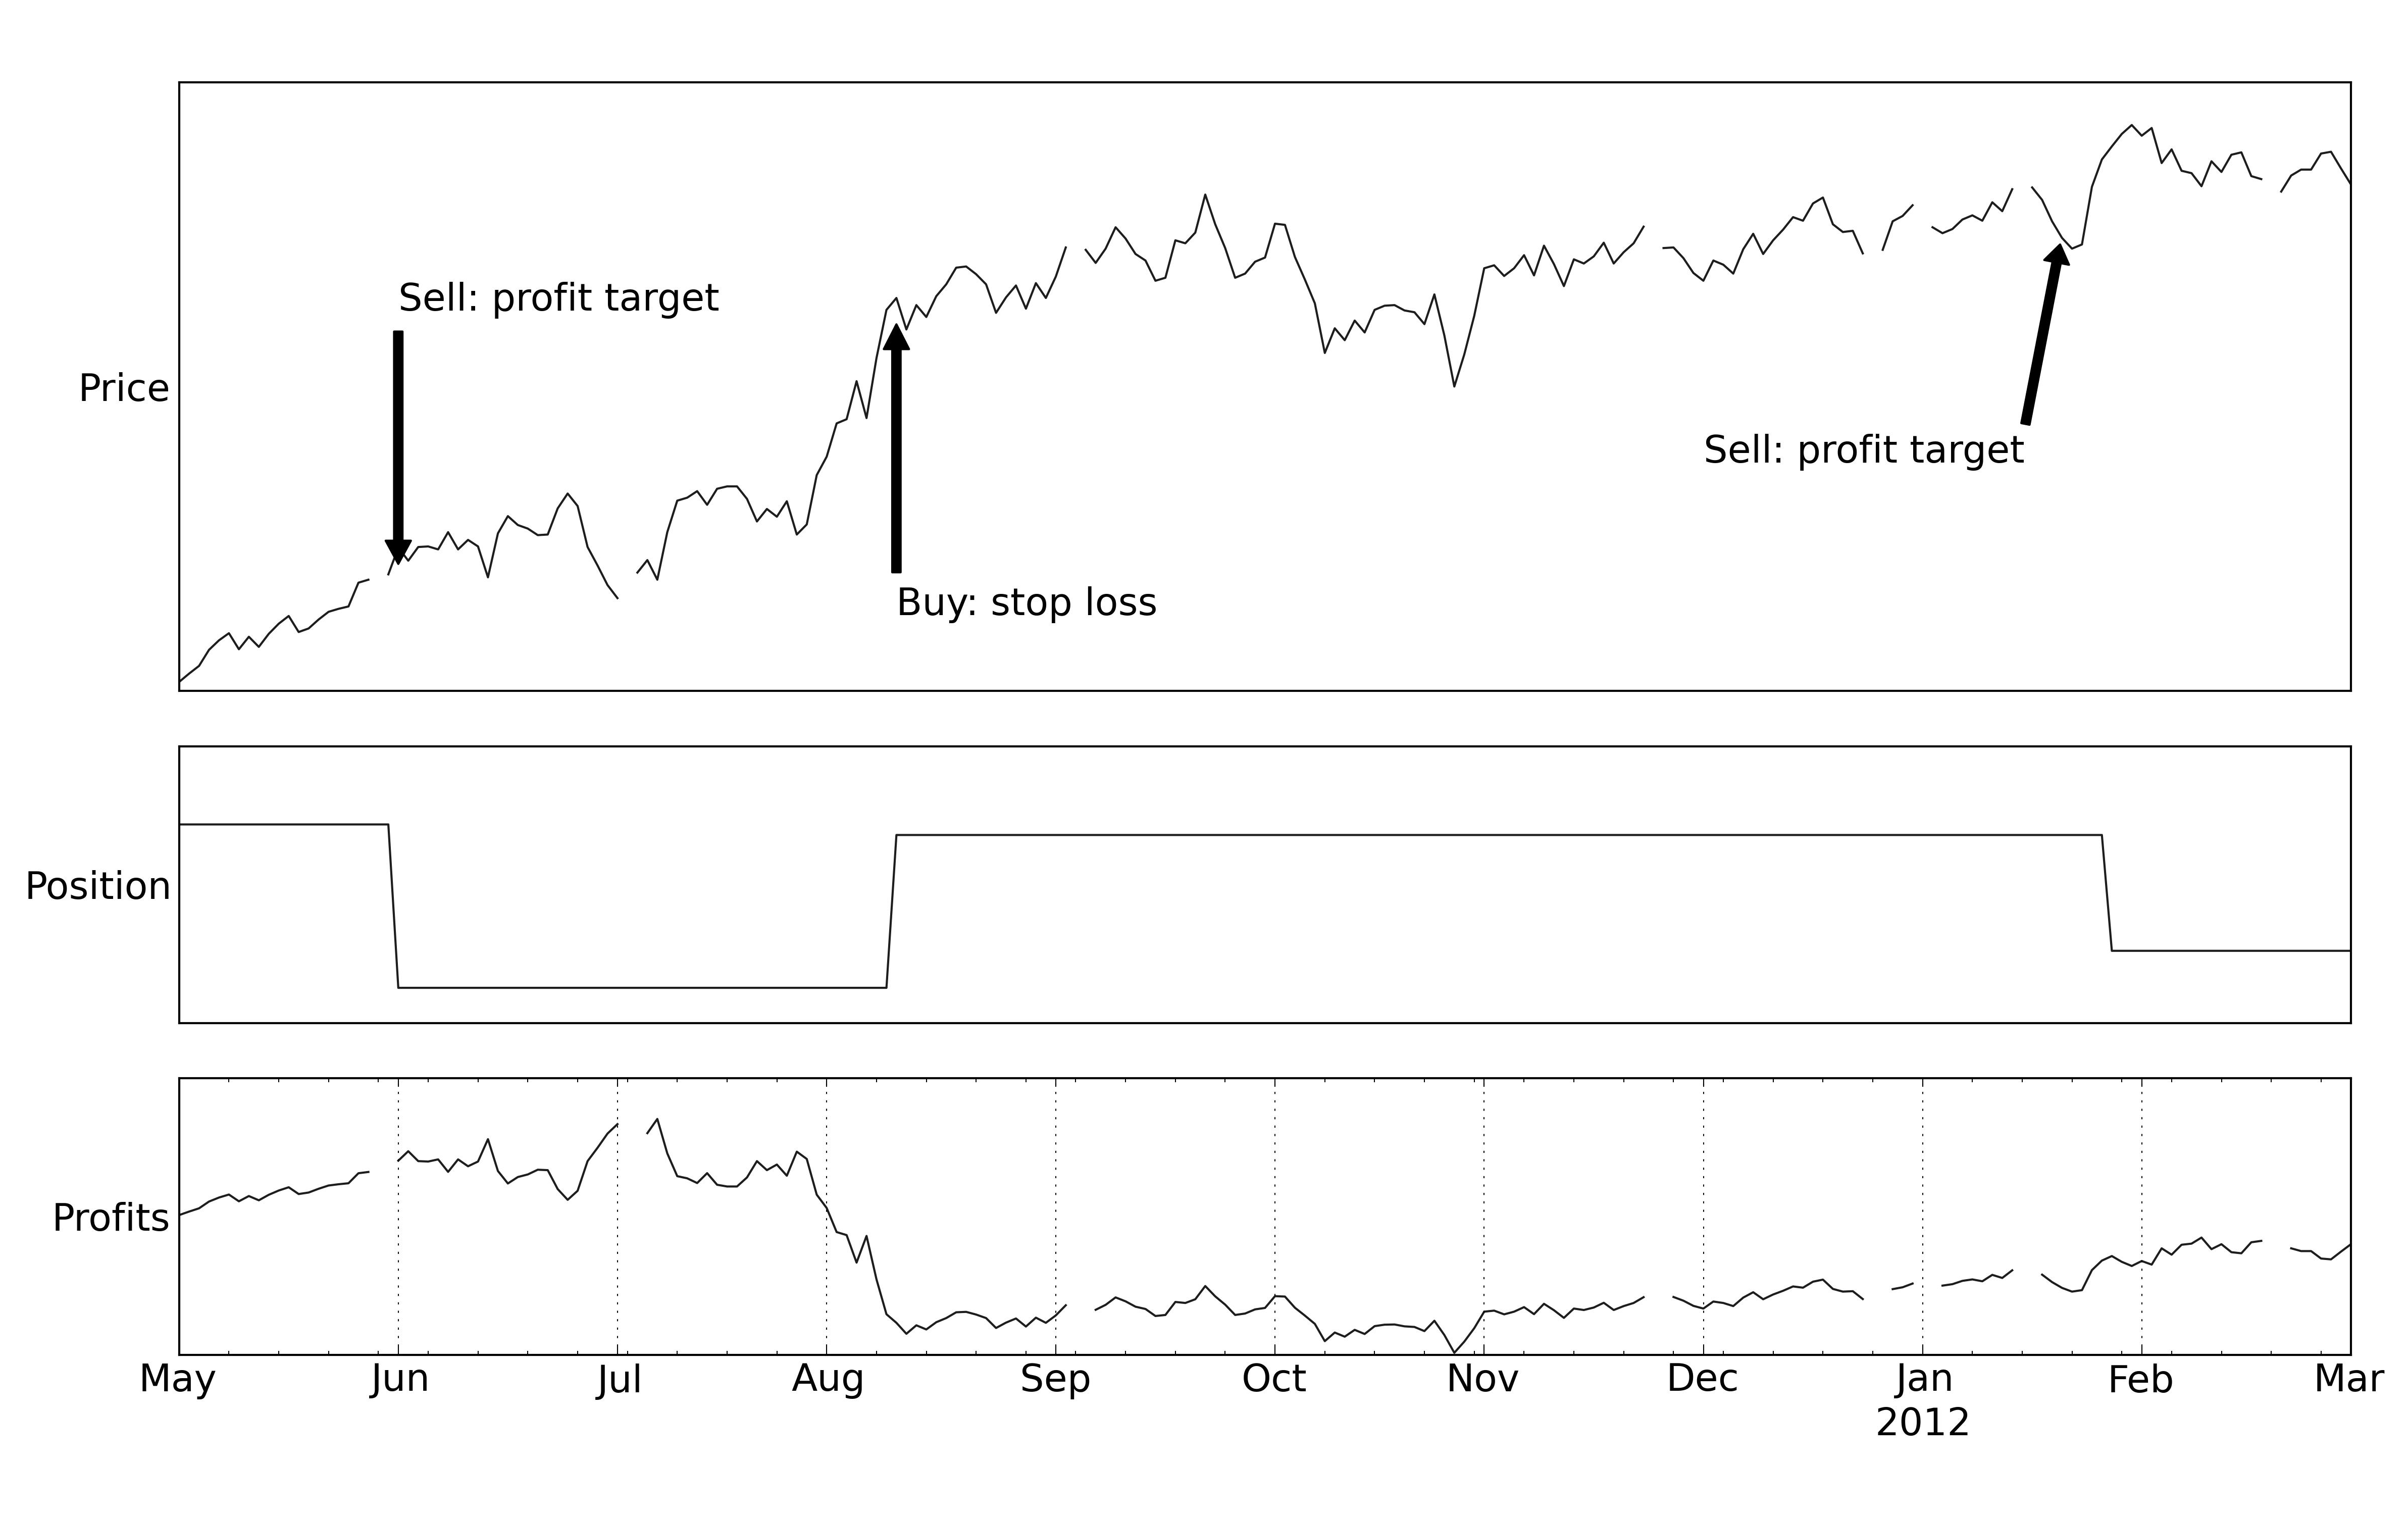
\includegraphics[width=\textwidth]{figures/raw/img-002.png}
  \caption{Early profit taker misses the 2011 rally in US 10 year treasury bonds.\\
  过早止盈者错过了 2011 年美国 10 年期国债的那波上涨。}
\end{figure}

I compared this to the results from employing the opposite strategy --- ``an early loss
taker''.\footnote{This is also based on the ``A and B'' system in appendix B with A = 20
and B = 5.\par 这同样基于附录 B 中的 “A and B” 系统，其中 A = 20，B = 5。} Figure 3 shows this rule did much better during the same time period.

我把它与另一种完全相反的策略进行了比较，也就是“过早止损者（early loss taker）”。图 3 显示，在同一时期，这条规则的表现要好得多。

\subsection*{CONCEPT: BACK-TEST}
\bisubsectiontitle{概念：回测}

To run a back-test you take historic data and calculate how a trading strategy would have
behaved, and the profits or losses it could have made, had you been using it in the past.

所谓回测，就是拿历史数据来计算：如果你过去一直在使用某个交易策略，它会如何运作，以及它本可能带来怎样的盈利或亏损。

Suppose you thought that buying the pound/dollar FX rate at 1.5 and selling it at 1.8 was
a profitable strategy. You could take the history of the FX rate and then see what trades,
and any profits, you would have made historically if you really had bought and sold
according to this rule.

假设你认为，在英镑兑美元汇率为 1.5 时买入、在 1.8 时卖出，是一个有利可图的策略。你就可以拿这条汇率的历史数据来检验：
如果你过去真的一直按这条规则买卖，那么历史上你究竟会做出哪些交易，又能赚到多少利润。

Back-testing is an invaluable tool for creating new trading rules. But when misused it can
be dangerous, as we'll discover in chapter three, ``Fitting''.

回测是创造新交易规则时极其宝贵的工具。但如果使用不当，它也可能很危险，正如我们会在第三章“拟合”中看到的那样。

\begin{figure}[htbp]
  \centering
  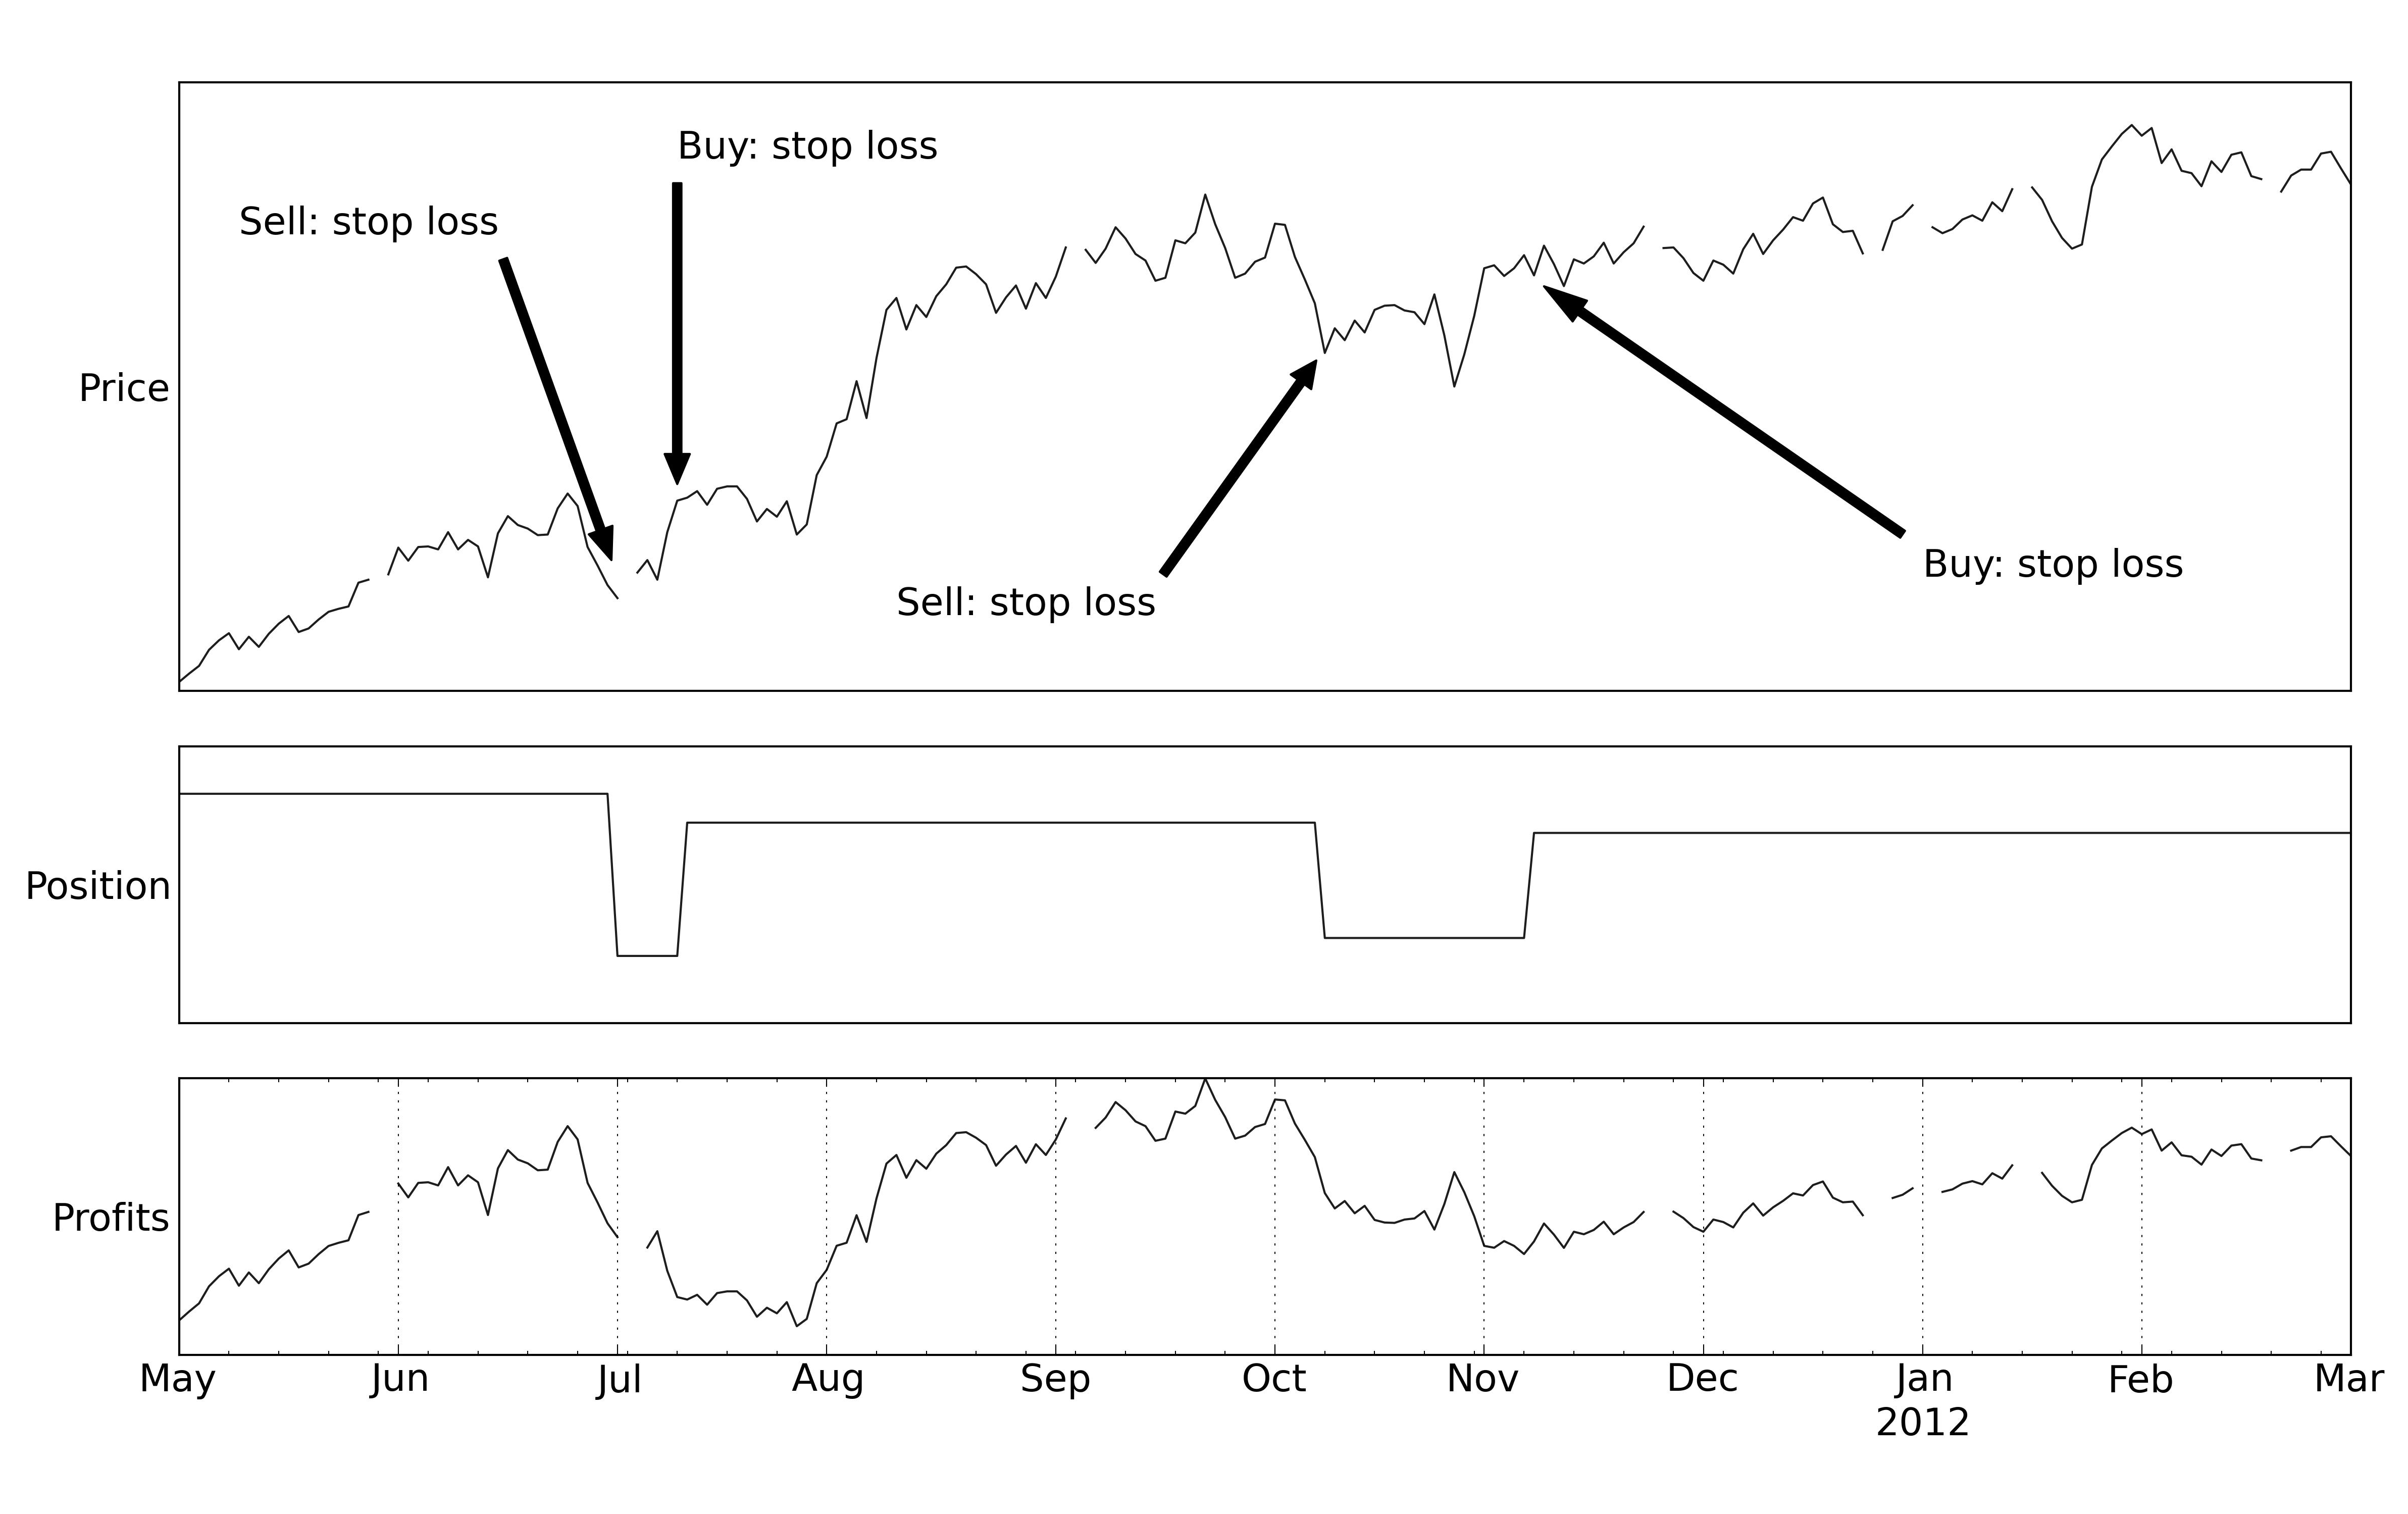
\includegraphics[width=\textwidth]{figures/raw/img-003.png}
  \caption{Early loss taker stays in the 2011 US bond rally until being stopped out.\\
  过早止损者一直持有 2011 年美国国债上涨行情，直到被止损离场。}
\end{figure}

When I back-tested these two rules on 31 futures contracts I found that the early loss
taker beat the early profit taker in 27 of them. Tests done on similar rules, across a wide
variety of asset classes, confirm this finding. The early profit taker rule, which mimics our
natural instincts, does worse than a rule which does the opposite.

当我在 31 个期货合约上回测这两条规则时，发现“过早止损者”在其中 27 个合约上的表现都胜过了“过早止盈者”。在各种资产类别上，
对类似规则所做的测试也都证实了这一发现。模仿我们天然本能的“过早止盈者”规则，表现反而不如与本能完全相反的那条规则。

\subsection*{Gamblers anonymous}
\bisubsectiontitle{赌徒互助会}

Some of my relatives equate trading to high stakes gambling; an attitude I am usually
quick to dismiss. But there may be some truth to it, at least in certain situations. To
understand why it's worth knowing that certain types of gambling are more addictive
than others, probably due to certain factors which reinforce the stimulation the brain
receives during play.

我的一些亲戚把交易等同于高风险赌博；通常我会立刻反驳这种看法。不过，这种说法在某些情境下或许确实有几分道理。要理解为什么，
我们需要知道：有些类型的赌博比另一些更容易让人上瘾，而这很可能是因为某些因素会强化大脑在赌博过程中所获得的刺激。

There appear to be three main factors associated with the most addictive games. Firstly
there should be an illusion of control, which encourages the perception of skill. Lottery
players often prefer to pick their own numbers. Secondly, the game should include
apparent near misses; frequent chances of almost winning the biggest prize. These are
especially potent if you also receive lower value prizes, as in lotteries and slot machines.
Finally, the game should be rapid and continuous to give a constant flow of stimulation.
Buying a lottery ticket is not as addictive as an instant lottery or scratch card where the
result is known immediately.

最容易让人上瘾的游戏，似乎都具备三个主要因素。第一，要让人产生一种控制幻觉，从而鼓励人们觉得自己拥有某种技巧。买彩票的人往往更喜欢自己选号。
第二，游戏中应当包含看似“差一点就中”的近失情形，也就是频繁出现几乎赢得大奖的机会。如果同时还会给出一些价值较低的小奖，
例如彩票或老虎机中的情况，这种效果会尤其强烈。最后，游戏应该节奏快速、连续不断，从而提供持续的刺激流。购买一张普通彩票，
就没有那种结果立刻揭晓的即开型彩票或刮刮卡那么容易让人上瘾。

\section*{Simple trading rules}
\phantomsection
\addcontentsline{toc}{section}{Simple trading rules}
\bisectiontitle{简单交易规则}

Given there are flaws in the human brain which seriously affect our decision-making
ability, what can we do about it? Easy: we should use systematic trading rules to make
our decisions. These can help mitigate our own serious flaws, but they can also allow us
to exploit the weaknesses that other human traders still have; their cognitive biases which
result in behavioural anomalies in the market.

既然人脑存在会严重影响我们决策能力的缺陷，那我们该怎么办？答案很简单：我们应该使用系统化交易规则来做决策。这样做不仅能帮助我们缓解自身的重大缺陷，
还能够让我们利用其他人类交易者仍然保有的弱点，也就是那些会在市场中造成行为异常的认知偏差。

For example the early loss taker rule I mentioned above isn't just correcting our human
instinct to take profits early and hang on to losses. It earns extra returns when other
people persist in doing the opposite.

比如我上面提到的“过早止损者”规则，不只是纠正了我们那种过早止盈、死扛亏损的人类本能。当其他人依旧坚持做相反的事情时，它还能因此赚到额外收益。

Personally I find it very reassuring to have explanations based on cognitive biases of why
certain trading rules are consistently profitable. This gives me confidence that what I am
seeing isn't just a statistical blip in a back-test. It means that the relevant rules should
continue to work unless human behaviour changes radically. I'll return to this theme in
chapter two --- ``Systematic Trading Rules''.

就我个人而言，如果某些交易规则为何能够持续盈利，能够用认知偏差来加以解释，这会让我感到非常安心。这会给我信心，让我相信自己看到的并不只是回测中的统计偶然。
这意味着，只要人类行为没有发生根本性改变，这些规则就应该继续有效。我会在第二章“系统化交易规则”中再次回到这个主题。

\section*{Sticking to the plan}
\phantomsection
\addcontentsline{toc}{section}{Sticking to the plan}
\bisectiontitle{坚持计划}

There is no point running a systematic trading strategy unless you can stick to it. Suppose
you make a New Year's resolution to follow the early loss taker rule. Like most such
resolutions it will probably prove hard to keep. When a long position in gold futures hits
the 5 cent stop loss the early loss taker rule has set you will probably start making excuses:

如果你根本做不到坚持执行，那么运行一套系统化交易策略就毫无意义。假设你在新年立志，要遵守“过早止损者”规则。和大多数新年决心一样，
它很可能很难真正坚持下去。当你持有的黄金期货多头头寸触及这条规则设定的 5 美分止损位时，你大概就会开始给自己找借口：

\begin{quote}
``The fundamentals are good. They haven't changed. I will just hold on a bit longer. Just
this once. If it goes down 10 cents --- which it won't --- then I will definitely sell.''
\end{quote}

\begin{quote}
“基本面还是好的，又没变。我就再多拿一会儿。就这一次而已。要是它再跌 10 美分 --- 虽然根本不会 --- 那我肯定卖掉。”
\end{quote}

You might not even close at a 10 cent loss, kicking yourself for not selling earlier, and
continue to hang on for the rebound that never comes, until the pain is unbearable and
you close out. A small profit would also prove irresistible, with its own litany of excuses
why you should deviate from the rule, just this once.

你甚至可能到了亏损 10 美分时也还是不平仓，一边责怪自己为什么没早点卖，一边继续死扛，等待那个永远不会到来的反弹，直到痛苦难以忍受才终于离场。
而如果出现一点小利润，它同样会显得难以抗拒，你又会为“这次偏离规则也没关系”找出另一整套理由。

I call this process of interference by our internal monologue meddling. Meddling is due
to the biggest cognitive bias of all: overconfidence. We think we are cleverer than the
trading system and we are. We think we know more than the trading system and we do;
the system focuses on a narrow set of quantifiable inputs, whilst we can analyse many
kinds of complex information. We think being clever and knowing more implies we will
make better decisions --- but we usually don't, thanks to cognitive biases.

我把这种被内心独白不断插手、偏离系统的过程称为“干预（meddling）”。干预源于所有认知偏差中最大的一种：过度自信。我们觉得自己比交易系统更聪明，
而且某种意义上也确实如此。我们觉得自己知道得比交易系统更多，而这也没错；系统只关注一组狭窄、可量化的输入，而我们却能够分析各种复杂信息。
于是我们便以为，更聪明、知道得更多，就意味着能做出更好的决定 --- 可由于认知偏差，事实通常并非如此。

To stop meddling with our trading systems we require what economists call a commitment
mechanism. The idea of a commitment mechanism is several thousand years old. One of
its earliest appearances is in the story of Odysseus. The mythical Greek wanted to hear the
songs of the Sirens without endangering himself or his vessel. So he ordered his crew to
stuff their ears with beeswax, tie him to the mast and dutifully ignore his inevitable cries
to steer the ship on to the rocks.

为了停止对交易系统的干预，我们需要经济学家所说的“承诺机制（commitment mechanism）”。承诺机制这个想法已经有几千年历史了，
它最早的典故之一就出现在奥德修斯的故事中。这位神话中的希腊英雄想要听海妖的歌声，同时又不让自己和船只陷入危险。于是他命令船员们用蜂蜡堵住耳朵，
把自己绑在桅杆上，并且无论他怎样哀求，都要坚决忽视他把船驶向礁石的命令。

A modern example of this is given in Victor Niederhoffer's book \textit{Education of a
Speculator}. At this point in the story hedge fund manager Victor has a large long position
in silver futures. We join him in early 1980 when the Hunt brothers, who had been
squeezing the market upwards, are about to capitulate, which will cause the price to
drop:

Victor Niederhoffer 的书 \textit{Education of a Speculator} 里提供了一个现代版本的例子。在故事进行到这一段时，
对冲基金经理 Victor 持有大量白银期货多头头寸。时间来到 1980 年初，之前一直在把市场往上挤压的 Hunt 兄弟即将投降，这会导致价格下跌：

\begin{quote}
``I decided to set my loss limit at 50\% of my winnings... The model story on this point
is Odysseus... I locked myself inside a racquetball court instead of tying myself to a ship's
mast. I issued instructions to my assistant and future wife, Susan. `Do not listen to my
entreaties if I wish to double further. If the losses reach 50\% of the winnings, reduce my
positions by one-half. If I beg to be released, sell everything out.'...

Some rumors about liquidation by the Hunts had hit the fan... I immediately placed a call
to Susan `Untie me. Disregard everything I said before' ... My faithful companion followed
my original directions.''
\end{quote}

\begin{quote}
“我决定把自己的亏损上限定在此前盈利的 50\%……在这个问题上，典型故事就是奥德修斯……我没有把自己绑在船桅上，而是把自己锁进了壁球场。
我对我的助手、也是未来的妻子 Susan 下达了指令：‘如果我想继续加倍，不要理会我的恳求。如果亏损达到此前盈利的 50\%，就把我的仓位减半。
如果我求你放我出来，那就把所有头寸全部平掉。’……

后来，关于 Hunt 兄弟清仓的传闻开始满天飞……我立刻给 Susan 打电话：‘给我松绑。把我之前说的话全都作废。’……我忠实的同伴遵照了我最初的指令。”
\end{quote}

Susan closed the entire position and Victor lived to fight another day. But how can we
ensure we stick to our strategies without the use of ropes or future wives?\footnote{This
comment isn't intended to imply that all investors and traders are unmarried heterosexual
men. However, if your partner is a man rather than a woman you should be wary of using
them as a commitment mechanism, as they may make things worse; research shows that
women generally make better investment decisions.\par 这句话并不是想暗示所有投资者和交易者都是未婚异性恋男性。不过，如果你的伴侣是男性而不是女性，
那么最好谨慎一点，不要把他们当作承诺机制，因为他们可能会让事情变得更糟；研究显示，女性整体上通常会做出更好的投资决策。}

Susan 最终把所有头寸都平掉了，Victor 因而得以活下来，继续迎接下一场战斗。但如果不靠绳子，或者不靠未来的配偶，我们又该如何确保自己能坚持执行策略呢？

\subsection*{Trading systems must be objective}
\bisubsectiontitle{交易系统必须是客观的}

To be committed you must have an objective trading system. Many systems aren't objective
and require some discretion to apply. A highly subjective rule would be something like
``Sell for small losses, and hold on to large profit making positions''. This is similar in spirit
to the early loss taker rule defined earlier, but it's much too vague.

要实现真正的承诺，你必须拥有一套客观的交易系统。许多系统其实并不客观，在应用时仍然需要某种主观裁量。一个高度主观的规则可能是这样的：
“小亏就卖，大赚就继续持有。”这在精神上和前面定义的“过早止损者”规则有点相似，但它实在是太模糊了。

At the first sign of a loss it's likely you will start to redefine what constitutes ``small'' to
justify not selling. Few systems are that poorly defined, but many have ``rules'' in them
which allow for a significant degree of subjective interpretation. Technical analysts rarely
agree on which patterns exist in a particular chart, and what should be done with them.

一旦刚出现亏损，你很可能就会开始重新定义什么叫做“小”，以此为自己不卖出找理由。很少有系统会糟糕到这样定义不清，但很多系统中确实存在某些“规则”，
允许相当大程度的主观解读。技术分析师往往很难就某张图表里到底出现了哪些形态、以及该如何据此操作，达成一致。

Creating a purely objective system is a powerful commitment mechanism. If you have a
subjective system and your instinct goes against it, then you'll soon be bending the rules.
But if everything is clearly defined it creates a line in the sand beyond which any deviation
is obvious. You cannot fool yourself that you are following a system if you blatantly ignore
objective rules.

建立一套纯粹客观的系统，是一种强有力的承诺机制。如果你的系统带有主观性，而你的直觉又恰好和它相冲突，那么你很快就会开始扭曲规则。
但如果一切都定义得清清楚楚，它就会在地上划出一条界线，任何越界都会变得显而易见。若你公然无视客观规则，就不可能再骗自己说你还在遵守某个系统。

Furthermore we can only produce back-tests for purely objective systems. You will see
why this is important later in the chapter.

而且，我们也只能对纯客观系统做回测。为什么这一点如此重要，你会在本章后面看到。

\subsection*{Automation --- the use of dogs in finance and engineering}
\bisubsectiontitle{自动化 --- 金融与工程中的狗}

Another advantage of objective systems is that they can be automated, and automation is a
good commitment mechanism. You can't automate subjective systems because computers
cannot eyeball trend lines on charts; they need firm statements like ``Buy if the 20 day
moving average is above the 40 day''. They cannot interpret commandments like ``Sell
once the pattern is triggered unless there is a firm sign of bullish volume'' without a clear
definition of both the pattern and the meaning of bullish volume.

客观系统的另一个优点，是它们可以被自动化，而自动化本身就是一种很好的承诺机制。你无法把主观系统自动化，因为计算机不能像人一样凭眼睛去看图表上的趋势线；
它们需要明确的表述，比如“若 20 日均线高于 40 日均线则买入”。对于“当某个形态触发时卖出，除非出现明显的看涨成交量信号”这类指令，
如果没有对“形态”和“看涨成交量”作出清晰定义，计算机根本无从理解。

So an objective system is one which a computer can run. But it does not mean a computer
must run it. You can run many trading strategies using pencil and paper, or relatively
simple spreadsheets, to calculate trades which you then execute manually. Certain kinds
of systems involving complex rules, faster trading frequencies or trading in large numbers
of instruments\footnote{Instrument is my term for something that you trade or invest in.
So a share of BP is an instrument, as is a corn future, and so is a spread bet on the
yen/dollar exchange rate.\par Instrument 是我用来指代“你所交易或投资的对象”的术语。所以，一股 BP 股票是一种 instrument，
一份玉米期货合约是一种 instrument，针对日元/美元汇率的点差投注也同样是一种 instrument。} would be very time-consuming, or impossible, to run without
automation. But for simpler systems automation isn't necessary. Full automation is also
problematic for discretionary semi-automatic traders, although they could automate their
position and risk management framework once they've made their trading decisions
manually.

因此，客观系统就是计算机能够执行的系统。但这并不意味着必须由计算机来执行。你可以用纸和笔，或者相对简单的电子表格，来运行许多交易策略，
算出应当做哪些交易，然后再手动执行。对于某些包含复杂规则、交易频率更高，或者需要同时交易大量标的的系统，如果不自动化，运行起来会非常耗时，甚至根本不可能。
但对于较简单的系统，自动化并不是必要条件。对于带有主观判断的半自动交易者来说，全自动也会有问题，尽管在他们手动作出交易决策之后，
仍然可以把仓位和风险管理框架自动化。

Furthermore automation doesn't stop meddling. Firstly, consider the degree of automation.
Having a system which requires a human to do the actual execution of automatically
generated trades is still prone to meddling. If the process is completely automated from
end to end then interference is harder. There is an old joke that the best systematic
trading setup consists of a computer, a man and a dog. The computer runs a fully
automated strategy, the man feeds the dog, and the dog bites the man if he touches the
computer.\footnote{This joke evolved from earlier jokes involving various kinds of hardware
rather than trading systems. It is generally attributed either to management theorist
Warren Bennis, or to employees of Bell labs.\par 这个笑话源自更早一些关于各种硬件设备的笑话，而非专指交易系统。
它通常被归因于管理学家 Warren Bennis，或贝尔实验室的员工。}

此外，自动化并不能彻底阻止干预。首先，要看自动化的程度。若一个系统虽然自动生成交易指令，却仍需要人工去实际下单，那它依旧容易被干预。
如果整个流程从头到尾都完全自动化，那么人为插手就会困难得多。有个老笑话说，最好的系统化交易配置由一台电脑、一个人和一条狗组成：
电脑运行全自动策略，人负责喂狗，而狗负责在这个人碰电脑时咬他。

Secondly, any good automated software would have ways to override it in an emergency.
If you desperately want to meddle then there will be frequent ``emergencies''. Automation
is of little help unless you have faith in your trading rules. A system which is fully
automated but not completely trusted is potentially lethal.\footnote{The HAL computer in
Arthur C. Clarke's \textit{2001: A Space Odyssey} is a good example of what happens when
you take automation too far and then don't trust the system.\par Arthur C. Clarke 的
\textit{2001: A Space Odyssey} 中的 HAL 电脑，就是把自动化推得太远、却又不真正信任系统后果的一个好例子。}
Any sane person would be
tempted to shut it down at the first sign of trouble. So automation aids commitment, but
it must be done with a well designed system in which you have full confidence.

其次，任何优秀的自动化软件都会提供在紧急情况下人工覆盖的方式。而如果你内心强烈地想干预，那么“紧急情况”就会频繁出现。
如果你对自己的交易规则没有信心，那么自动化其实帮不了你多少。一个已经完全自动化、却没有被完全信任的系统，潜在上是致命的。
任何理智的人，在它刚出现一点异常时都会忍不住想把它关掉。因此，自动化确实有助于建立承诺，但前提是它必须建立在一套设计良好、且你完全信任的系统之上。

\section*{Good system design}
\phantomsection
\addcontentsline{toc}{section}{Good system design}
\bisectiontitle{良好的系统设计}

So what is a well designed system? How can you make something which you can trust,
commit to and won't meddle with, regardless of whether it is automated or not?

那么，什么才算是一套设计良好的系统？无论它是否自动化，你要怎样才能做出一套自己愿意信任、愿意承诺遵守、并且不会总想去干预的系统？

It is much easier to trust a system which is objective. Firstly, because it is transparent: you
know given some particular data exactly what the positions should be. Secondly, you can
back-test an objective system over history. This will give you an indication of what its
past behaviour was, and how it should trade in the future. For example suppose a system
typically lost around 5\% on one of every ten trading days in the simulated past of your
back-test. You shouldn't worry if in real trading you lose 5\% every couple of
weeks.\footnote{In fact by using my framework you can make predictions about likely
losses even in situations when you can't back-test, such as when you're a semi-automatic
trader not using systematic trading rules.\par 事实上，使用我的框架，即便在你无法做回测的情况下，
例如你是一个并未使用系统化交易规则的半自动交易者，也可以对可能的亏损作出预测。}

客观的系统更容易被信任。首先，因为它是透明的：面对给定的数据，你能确切知道仓位应该是什么。其次，你可以对客观系统进行历史回测。
这会让你知道它过去大致是如何表现的，以及未来大致该怎样交易。比如说，假设在你的回测模拟中，这套系统平均每 10 个交易日就会有 1 天亏损大约 5\%，
那么如果真实交易中你每隔两周左右亏 5\%，你就不该过度担心。

As well as requiring systems to be objective I also prefer those that are relatively simple,
transparent and based on underlying ideas,\footnote{Compared to say a system which has
been built purely by back-testing a large number of trading rules and picking the best
regardless of whether it can be explained, a process sometimes called data mining. I'll
return to this distinction in the next chapter.\par 这与那种纯靠回测大量交易规则、然后不管是否能解释都只挑表现最好的系统不同，
这种过程有时被称为“数据挖掘”。我会在下一章再次回到这个区别。} such as my previous hypothesis that
prospect theory explains the success of the early loss taking rule. Transparency is important
for gaining trust in trading systems, just as it is in politics. In the next chapter I'll explain in
more detail why I prefer systems whose performance and behaviour can be explained.

除了要求系统必须客观之外，我也偏好那些相对简单、透明，并且建立在底层逻辑之上的系统。比如我前面提出的假设：前景理论能够解释“过早止损者”规则为何成功。
透明性之所以重要，是因为它有助于建立对交易系统的信任，正如它在政治领域同样重要一样。下一章中，我会更详细地说明，
为什么我偏爱那些其表现和行为都能够被解释清楚的系统。

In addition to these positive attributes there are also three significant pitfalls to avoid when
designing trading systems: over-fitting, overtrading and over-betting.

除了这些正面特征之外，在设计交易系统时，还有三个必须避开的重大陷阱：过拟合、过度交易和过度下注。

\subsection*{Over-fitting}
\bisubsectiontitle{过拟合}

A new trading system does not arrive out of the ether. It has to be designed and developed
by an actual, probably overconfident,\footnote{It's not just trading system designers who are
overconfident. There is a significant amount of academic research showing examples of
overconfidence in discretionary finance, for example amongst equity analysts and
macroeconomic forecasters.\par 过度自信的并不只是交易系统设计者。大量学术研究都展示了主观金融判断中的过度自信现象，
例如股票分析师和宏观经济预测者身上就经常能看到。} person. It is all too easy for that person to make design
mistakes due to those same cognitive biases they are trying to escape from by trading
systematically.

一套新的交易系统并不会凭空从天而降。它必须由一个真实的人来设计和开发，而这个人很可能本身就过度自信。于是，这个人非常容易因为那些自己正试图通过系统化交易来逃避的认知偏差，
反而在设计阶段犯下错误。

Firstly ``narrative fallacy'': our brains are great at seeing patterns where there are none.
Whilst developing trading rules there is often a fitting process during which the best rules
are selected by looking at back-test results. If we're not careful the rules selected will fit the
data too well. They will be highly tuned to one set of market conditions and perform
worse in actual trading than a simpler rule would. The system will be over-fitted.

第一个偏差是“叙事谬误（narrative fallacy）”：我们的大脑非常擅长在根本不存在模式的地方看出模式。在开发交易规则时，
通常会有一个拟合过程，人们会根据回测结果来挑选“最好的”规则。如果我们不够小心，最终选出来的规则就会对数据拟合得过于完美。
它们会被高度调教到只适用于某一组市场条件，结果在真实交易中的表现反而不如更简单的规则。这样的系统，就是过拟合的。

Narrative fallacy means we have a tendency to see more predictability in historic asset
prices than really existed and so we're naturally drawn to over-fitted trading rules. I'll
return to this problem in chapter three, ``Fitting''.

叙事谬误意味着，我们倾向于在历史资产价格中看到比实际存在更多的可预测性，因此会自然而然地被那些过拟合的交易规则吸引。我会在第三章“拟合”中再次讨论这个问题。

Second bias, and perhaps the most serious of all: overconfidence. This manifests itself in
a lack of diversification. Surveys of individual portfolios find that most amateur investors
have relatively few securities in their portfolio, with a bias towards their home country,
and also lack diversification across asset classes.

第二个偏差，也许是最严重的一个：过度自信。它通常表现为缺乏分散化。对个人投资组合的调查发现，大多数普通投资者的组合中只持有相对较少的证券，
而且明显偏向本国市场，同时在资产类别之间也缺乏分散。

You might think that experts, with access to sophisticated quantitative tools, wouldn't
make these mistakes. Unfortunately they often do. This happens when they don't consider
the considerable uncertainty in expected asset returns. The most commonly used
optimisation models assume they know the pattern of returns precisely. Small changes to
the model inputs will produce extreme portfolios with all their eggs in one or two baskets.
The result can be just as bad or worse than the portfolios of mere amateurs.

你可能会以为，掌握复杂量化工具的专业人士不会犯这种错误。遗憾的是，他们经常也会。问题出在他们没有认真对待预期资产收益所包含的巨大不确定性。
最常用的优化模型，通常假设自己能够精确知道收益模式。这样一来，只要模型输入稍有变化，就会产生极端的投资组合，把所有鸡蛋几乎都放进一两个篮子里。
结果可能和普通业余投资者的组合一样糟，甚至更糟。

In practice many experts fiddle with the raw output of optimisations until they end up
reflecting their own expectations of what the result should have been! I will discuss this
further in chapter four, ``Portfolio Allocation''.

在现实中，很多专家会不断篡改优化模型的原始输出，直到结果最终看起来符合他们自己原本期待的样子！我会在第四章“投资组合配置”中进一步讨论这个问题。

\subsection*{Overtrading}
\bisubsectiontitle{过度交易}

People are highly overconfident about their own abilities relative to others. This is
another cognitive bias: illusory superiority. For example nearly all drivers consider
themselves above average, a theoretical impossibility and also highly unlikely given the
number of deaths annually from road accidents.

人们对于自己相对于他人的能力，通常都极度自信。这又是一种认知偏差：虚幻优越感（illusory superiority）。例如，几乎所有司机都会觉得自己的驾驶水平高于平均线，
这在理论上根本不可能成立；而考虑到每年因交通事故死亡的人数，这种想法在现实中也极不可信。

Both amateur investors and professional managers have a tendency to trade too
frequently.\footnote{For academic research on this see Odean and Barber, ``The common
stock investment performance of individual investors'', 1998 working paper.\par 关于这一点的学术研究，可参见 Odean 和 Barber 的 1998 年工作论文
“The common stock investment performance of individual investors”。} There are
extra costs involved in trading more often. Overtrading suggests overconfidence in your
own relative ability to overcome the higher hurdle of bigger costs.

无论是普通投资者还是专业管理人，都有过度频繁交易的倾向。交易越频繁，附带的成本也就越高。过度交易本身就意味着，
你对自己能跨越更高成本门槛的相对能力过于自信。

As I pointed out above, frequent trading can also be addictive and lead to behaviour which
is indistinguishable from problem gambling.

正如我前面指出的那样，频繁交易也可能让人上瘾，进而演变成与赌博成瘾几乎无法区分的行为。

When designing trading systems if you over-fit you will end up with systems that perform
unrealistically well in back-tests, and wrongly assume that returns will easily be high
enough to overcome trading costs.

在设计交易系统时，如果你过拟合，就会得到那些在回测中表现不切实际地优秀的系统，并错误地以为真实收益会轻而易举地高到足以覆盖交易成本。

\subsection*{Over betting}
\bisubsectiontitle{过度下注}

It will be extremely difficult to refrain from meddling if you're worried about wiping out
your capital. Take the system I mentioned above with a one-in-ten chance of a 5\% daily
loss. If that was ten times leveraged you would have a 10\% chance of losing half your
capital on any given day. Most sane people would panic after losing 50\% on one day, and
start meddling like crazy.

如果你一直担心本金会被亏光，那么想不去干预系统就会变得极其困难。还是以上面提到的系统为例：它大约有十分之一的概率在单日亏损 5\%。
如果你给它加上 10 倍杠杆，那么你在任意一天都有 10\% 的概率亏掉一半本金。绝大多数理智的人在一天之内亏掉 50\% 后都会立刻恐慌，
然后开始疯狂干预系统。

Unfortunately over betting is endemic amongst amateur investors with easy access to
leverage through derivatives like spread bets. If your confidence is unbounded you can
bet the maximum that your broker allows you to. Potentially this could be a ten-fold
leverage on an individual equity bet, equating to an annual standard deviation of returns
of around 200\%. This is nuts.\footnote{At the time of writing some UK providers of FX
spread bets offer leverage of up to 500 times. That isn't nuts, it's clinically insane.\par 在我写作本书时，
英国某些外汇点差投注提供商给出的杠杆最高可达 500 倍。那已经不只是疯狂，而是临床意义上的精神失常。}

遗憾的是，过度下注在那些可以通过点差投注等衍生品轻易获得杠杆的普通投资者中，几乎已经成了常态。如果你的自信心没有边界，
你完全可以下注到经纪商允许的最大规模。这在单只股票的交易上，可能意味着 10 倍杠杆，对应的年化收益标准差大约会达到 200\%。这简直疯了。

\subsection*{CONCEPT: STANDARD DEVIATION}
\bisubsectiontitle{概念：标准差}

The standard deviation is a measure of how dispersed some data is around its average; it's
a measure of risk. The precise formula is in the glossary, but in most cases you'll use a
spreadsheet formula or software to calculate it.

标准差衡量的是一组数据围绕其平均值的离散程度；它也是一种风险度量。精确公式可以在词汇表中找到，但在大多数情况下，
你会直接用电子表格公式或软件来计算它。

Standard deviations are often used to describe the dispersion of the returns of an asset, or
profits from a trading system. I use the term volatility as a shorthand for standard deviation
of returns. One unit of standard deviation is also sometimes called a sigma.

标准差常被用来描述某项资产收益，或某套交易系统利润的离散程度。我会把“波动率（volatility）”作为“收益标准差”的简称来使用。
一个标准差单位有时也会被称为一个 sigma。

In this book we'll usually be dealing with daily returns and using daily volatilities, but it's
often useful to think about the annualised standard deviation --- how much deviation we
expect to see over a year.

在本书中，我们通常处理的是日收益，并使用日波动率，但很多时候从年化标准差的角度来思考会更方便，也就是我们预计在一年内会看到多大的波动幅度。

Standard deviation doesn't increase linearly, but with the square root of time. Over the
roughly 256 business days in a year you'd expect annual standard deviation to be larger by
the square root of 256, or 16.\footnote{I'm making an assumption here that adjacent returns
don't influence each other, or in the jargon of statistics they have zero autocorrelation.\par 这里我做了一个假设，
即相邻收益之间互不影响；用统计学术语来说，就是它们的自相关为零。} So
you multiply daily standard deviations by 16 to get the annualised version, or divide by 16
to go from annualised to daily.

标准差并不会线性增长，而是按时间的平方根增长。一年大约有 256 个交易日，因此你可以预期年化标准差会比日标准差大上 $\sqrt{256}$ 倍，也就是 16 倍。
所以，从日标准差换算成年化标准差时，你要乘以 16；反过来，从年化换算到日度时，则要除以 16。

In contrast to go from average daily returns to annualised average returns you just multiply
by the number of days in a year, or 256. Then to go from annualised to daily you divide by
256.

相反，从平均日收益换算成年化平均收益时，只需要乘以一年中的天数，也就是 256。反过来，从年化换算到日度，则除以 256。

Equities have an annualised standard deviation of about 20\% a year. Bonds tend to be
safer, depending on their maturity. A typical two year bond has an annualised sigma of
around 1.5\% a year, and a ten year bond would be more like 8\%.

股票的年化标准差大约是每年 20\%。债券通常更安全一些，当然也取决于其期限。一个典型的两年期债券，其年化 sigma 大约在每年 1.5\% 左右；
而十年期债券则更接近 8\%。

We often assume our returns have a particular type of distribution. A distribution is just a
way of describing the pattern of your data. A common distribution I use is the Gaussian
normal distribution. If returns are Gaussian normal, then the mean and standard
deviation alone are sufficient to say how likely certain returns will be.

我们常常会假设收益服从某一种特定的分布。所谓分布，只是描述你的数据呈现何种模式的一种方式。我常用的一种分布是假设收益服从高斯正态分布。
如果收益是高斯正态的，那么仅凭均值和标准差，就足以说明某些收益出现的概率有多大。

If your daily returns are Gaussian normal then you will see movements one sigma or less
around the average about 68\% of the time, and returns two sigma or less about 95\% of
the time. In 2.5\% of days you'd see a change more than two sigma above the average.
You'd also see a return which is two sigma worse than the average 2.5\% of the time. The
Gaussian normal distribution is symmetric.

如果你的日收益服从高斯正态分布，那么大约有 68\% 的时间，收益会落在均值上下一个 sigma 以内；大约有 95\% 的时间，会落在两个 sigma 以内。
在 2.5\% 的交易日里，你会看到高于均值两个 sigma 以上的变化；同样地，也会有 2.5\% 的时间出现低于均值两个 sigma 以上的收益。高斯正态分布是对称的。

Let's consider the 200\% annualised standard deviation mentioned above. 200\% a year
translates into 12.5\% a day if you divide by the square root of time, 16. For the average
daily return even if you're making an optimistic 200\% a year, after you've divided by 256
you earn just 0.8\% per day. A plus one sigma return would be 12.5\% above the average
of 0.8\%, or 13.3\%. A one sigma loss would be 12.5\% below the average, or -11.7\%.

让我们来看前面提到的 200\% 年化标准差。按时间平方根 16 去除之后，200\% 的年化波动相当于日波动 12.5\%。至于平均日收益，
即便你非常乐观地认为年收益能达到 200\%，除以 256 之后，每天也不过只有 0.8\%。那么一个正向一个 sigma 的收益，就是在 0.8\% 的平均值之上再加 12.5\%，
也就是 13.3\%；而一个负向一个 sigma 的损失，则是在平均值之下减去 12.5\%，也就是 -11.7\%。

\begin{figure}[htbp]
  \centering
  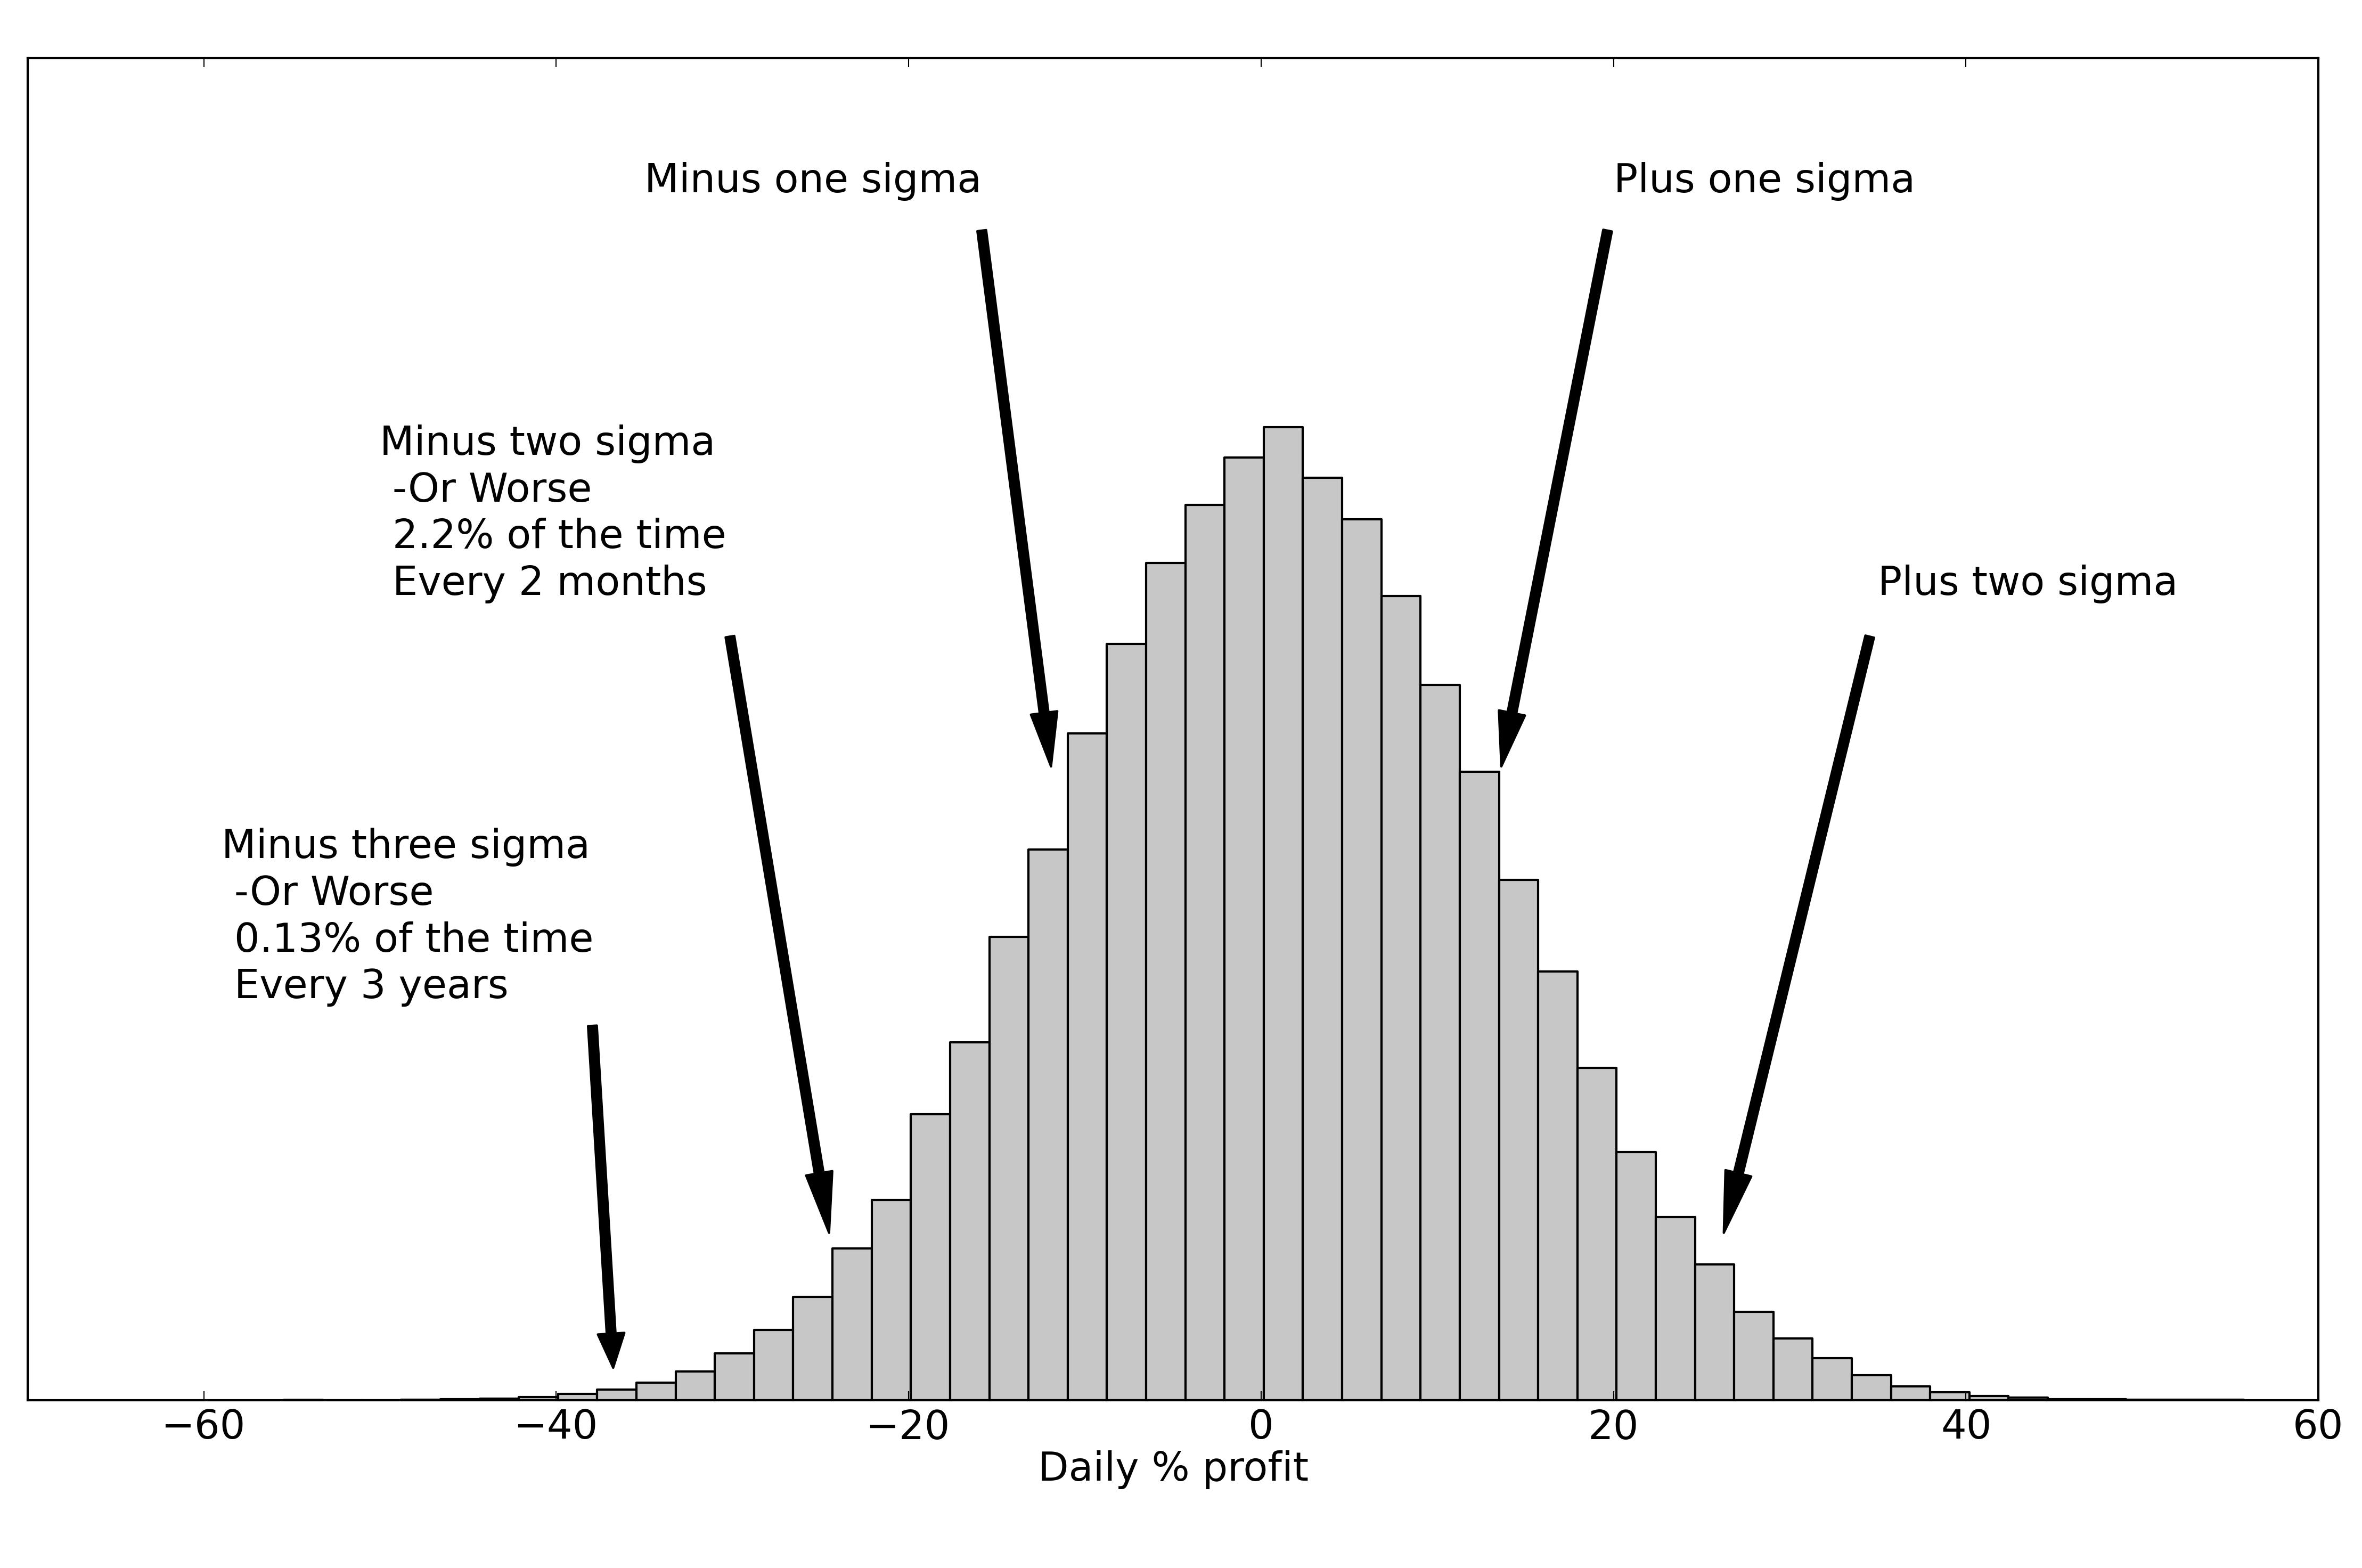
\includegraphics[width=\textwidth]{figures/raw/img-004.png}
  \caption{Scarily you can expect to lose 40\% in one day, every three years, for a trading
  system with 200\% annualised standard deviation of returns, and average returns of
  200\% per year.\\
  很可怕的是，对于一个年化收益标准差为 200\%、平均年收益也为 200\% 的交易系统，你可以预期大约每三年就会在单日亏掉 40\%。}
\end{figure}

You'll see returns between -11.7\% and +13.3\% a day around 68\% of the time, and
between -24.2\% and +25.8\% a day 95\% of the time. Around 2.5\% of the time you'd
see losses of more than 24.2\% a day. That's quite a hefty daily loss which you'd get every
couple of months. And as figure 4 shows about once every three years you'd lose three
sigma or 37.2\% in one day!

大约有 68\% 的时间，你会看到日收益落在 -11.7\% 到 +13.3\% 之间；大约有 95\% 的时间，则会落在 -24.2\% 到 +25.8\% 之间。
而大约 2.5\% 的时间里，你会在一天之内亏掉超过 24.2\%。这已经是相当沉重的单日亏损了，差不多每隔几个月就会发生一次。更可怕的是，正如图 4 所示，
大约每三年你就会在一天之内亏掉三个 sigma，也就是 37.2\%！

Scarily that's probably still optimistic because the normal distribution tends to
underestimate the chance of really bad returns. According to the normal distribution we
should get daily falls of more than 4 sigma about once a century. But from 1914 to 2014
the US Dow Jones index fell by more than 4 sigma around 30 times!

可怕的是，这样的估计可能仍然偏乐观，因为正态分布往往会低估真正极端坏结果出现的概率。按照正态分布，我们本应大约每一百年才遇到一次超过 4 sigma 的单日下跌。
但从 1914 年到 2014 年，美国道琼斯指数却出现了大约 30 次超过 4 sigma 的下跌！

You or your investors need to be comfortable with the losses you're likely to make. The
size of your positions must reflect the amount of risk you can handle. I'll explain this in
more detail in chapter nine, ``Volatility Targeting''.

无论是你自己还是你的投资者，都必须能够接受这种可能发生的亏损。你的仓位大小，必须反映你所能承受的风险水平。我会在第九章“波动率目标”中更详细地解释这一点。
